\textit{This section complements this work presenting an example of applications of some concepts presented in this thesis.}

\section{Detecting Erroneous Link candidates in Educational Link Repositories}

\textit{Interlinking educational datasets is a challenging task when the majority of data is not organized in a Linked Data standards. Thus, we face data that is not well interlinked among several different datasets of the educational area. This task usually involves many steps such as Link Discovery, where links across homogeneous datasets are discovered and stored, and quality assessment of these links, where the consistency of these links is verified. 
    However, a large number of these links are erroneous and can thus lead to these applications producing absurd results.
    The aim of this paper is to provide a way to check the consistency of linksets from Educational area. To this end, we are using an approach called CEDAL which is a time-efficient and complete approach for the detection of erroneous links for properties that are transitive.
    In order to evaluate our approach we selected $1,049$ transitive from linksets from Nature.com, Geonames, educational Programs, among others.}

\subsection{Introduction}
%\todo[inline]{Objective: Verify weather linksets from Educational area are Consistent.}
Links across knowledge bases play a fundamental role in Linked Data~\cite{Albertoni:2013:ALQ:2457317.2457327} as they  allow users to navigate across datasets, integrate Linked Data sources~\cite{NgomoSL14}, perform federated queries~\cite{saleem2013daw} across data sources and perform large-scale inference on the data.
Given the importance of links, corresponding repositories such as \emph{nature.com}\footnote{\url{http://nature.com/}} and LinkLion~\cite{nentwig2014linklion} have been created. 
In addition to facilitating the finding of links between  resources and knowledge bases, these repositories also allow detecting significant errors across links. 
For example, according to Nature.com and by virtue of transitivity, the resources. \texttt{http://purl.org/spar/fabio/ExpressionCollection} and \texttt{http://purl.org/ontology/bibo/Collection} stand for the same entity of the real world but have different URIs within the same knowledge base. 
This clearly goes against the definition of URIs as used in RDF.

figure \ref{fig:example} shows a fictional example to help illustrate such problems, which can be classified as \textbf{contradiction problems}, according to the quality dimension of consistency~\cite{zaveri2015quality}. 
In our example, we can infer that one of the links along the path that led to this inference is wrong or that the knowledge base in itself contains an error. 

Educational data needs to be enriched, that is transformed into structured and formal descriptions by linking it to widely established Linked Data vocabularies and datasets on the web also linking these datasets in a efficient way in order to avoid redundancy.

In this context we found linksets from Nature.com, Educational Programs\footnote{\url{https://datahub.io/dataset/educationalprograms_sisvu}} and Geonames, in which such errors can be potentially detected by computing the closure of equivalence links using the characteristics of equivalence relations and an inference engine. In our case we are using CEDAL \cite{cedal2017} which is the fastest and complete way to detect consistency errors. 

\begin{figure*}[htb] 
	\centering
	\includegraphics[width=1.0\linewidth]{img/example8.pdf}
	\caption{Manual detection of erroneous resource candidates.}
	\label{fig:example}
\end{figure*} 

\subsubsection{Research questions}

The research questions are:
\begin{itemize}
    \item The link repositories from the educational area are consistent?
    \item Is there an approach to verify whether the links from educational area are consistent?
\end{itemize}


\subsubsection{Our contributions}
\begin{itemize}
    \item An analysis of linksets from educational area.
    \item Applying CEDAL\cite{valdestilhas2017cedal} in order to assess the consistency of linksets from educational area.
\end{itemize}

\subsection{Related works}

Works such as \cite{rajabi2015interlinking,dietze2013interlinking,Dietze:2012:LEI:2245276.2245347} present an effort to interlinking educational resources into linked data standards, but without taking care of the problem of the consistency of the linksets.

The work presented in \cite{d2013assessing} is a research note about a study of available web datasets related to education. They focus in a network of educational web data. The common point is that part of the analysis is about of \texttt{owl:sameAs} links from education area and the novelty of our work is about we are taking care about linksets and not only datasets.
    
There is a study more generic and comprehensive about Linked Data for science in general and education \cite{kessler2013linked}, in which makes an introductory analysis of four papers documenting the most recent developments in Linked Data for Science and Education.

We found a work about Information and Communication Technologies (ICT) tools to support learning activities with a Linked Data approach for the discovery of educational ICT tools in the Web of Data \cite{ruiz2012linked}, in which proposes to collect data from third-party sources, align it to a vocabulary understandable by educators and finally publish it to be consumed by educational applications. The relation here is the effort to turn educational data in linked data and improve the quality.

The work \cite{zablith2011linked} has the aim of introduce the current efforts toward the release and exploitation of The Open University’s (OU) Linked Open Data (LOD) referring to production and consumption. The relation here is about bring some improvement to the educational linked data, but without taking care of quality of linksets.

\subsection{Preliminaries} \label{preliminaries}

%We now introduce the terminology and symbolism that is used throughout the rest of this paper.

%Also, a base concept of our work comes from the Ancient Greek, about the syllogism created by Aristotle where \textit{if} $ A=B$\textit{, and} $B=C$\textit{, then} $A=C$. Thus, from this definition we have a bridge to the concept of transitive closure.

\begin{description}
% \item[\textbf{RDF graph.}] An RDF graph is a set of RDF triples which has a set of subjects and objects of triples in the graph called nodes.
% Given an infinite set $U$ of URIs, an infinite set $B$ of blank nodes and an infinite set of literals $L$, a RDF triple is a triple $\langle s, p, o \rangle$ where the subject $s \in (U \cup B)$, the predicate $p \in U$ and the object $o \in (U \cup B \cup L)$. An RDF triple represents an assertion of a ``piece of knowledge'', so if the triple $\langle s, p, o \rangle$ exists, then,  the logical assertion $p(s,o)$ holds true.

% An RDF graph is also represented by a collection of RDF triples and it can be seen as a set of statements describing, partially or completely, a certain knowledge.

\item[\textbf{Transitive property.}] Defined by: $\forall a,b,c \in X:(aRb \wedge bRc) \implies aRc$, where $R$ represents a relation between two elements of a set $X$.

%\item[\textbf{Antisymmetric property.}] Defined by $\forall a,b \in X:(aRb \wedge bRa) \implies a=b$, where $R$ represents a relation between two elements of a set $X$. \todo{TS: Do we still need this?}

\item[\textbf{Equivalence.}] An equivalence relation $\equiv$ is a binary relation that is reflexive, symmetric and transitive. According to OWL semantics, \texttt{owl:sameAs} is an equivalence relation.

\item[\textbf{Linkset.}]
According to the W3C,\footnote{\url{https://www.w3.org/TR/void/\#linkset}} a linkset is a collection of RDF links between two datasets. It is a set of RDF triples in which all subjects are in one dataset and all objects are in another dataset. RDF links often have the \texttt{owl:sameAs} predicate, but any other property could occur as the predicate as well.
Formally, according to \cite{alexander2009describing}, a linkset $LS$ is a set of $RDF$ triples where for all triples $t_i =  \langle s_i, p_i, o_i \rangle \in LS$,  the subject is in one dataset,  i.e. all $s_i$ are described in $S$, and the object is in another dataset, i.e. all $o_i$ are described in $T$.

We use the word \emph{linkset} for either RDF knowledge base files and dump files from RDF link repositories.

\item[\textbf{RDF graph partitioning.}]
Given a graph $G=(V,E, lbl, L)$, a graph partitioning, C, is a division of $V$ into $k$ partitions ${P_1,P_2,...,P_k}$ such that $\bigcup\limits_{1 \leq i \leq k}P_i=V$, and $P_i \cap P_j = \emptyset$ for any $i \neq j$. The edge cut $E_c$ is the set of edges whose vertices belong to different partitions, $lbl : E \cup V \rightarrow L$ is a labeling function, and $L$ is a set of labels. 


%\begin{figure}[H] 
%	\centering
%	\includegraphics[width=300pt]{img/graphPartitioning}
%	\caption{A example of graph partitioning.}
%	\label{fig:graphPartition}
%\end{figure}

The definition comes from a recent survey about RDF graph partitioning~\cite{tomaszuk2015rdf}.

\item[\textbf{Error Types.}]

This paper uses two types of errors defined in \cite{cedal2017}. (1) \textbf{Semantic accuracy} errors, in which we detect if data values correctly represent the real world facts. (2) \textbf{Consistency} and \textbf{Conciseness} errors where a knowledge base is free of logical or formal contradictions concerning particular knowledge representation and inference mechanisms and the minimization of redundancy of entities at the schema and the data level. 
figure \ref{fig:errorType} shows a fictional example of both error types, in which we represent links between  GeoNames\footnote{\url{http://www.geonames.org/}} and DBpedia.\footnote{\url{http://dbpedia.org/}}

\begin{figure}[H]
	\centering
	\subfigure[Error type (1).] 
	{
		\includegraphics[width=0.4\linewidth]{img/CEDAL1_2.pdf}
		\label{fig:error1}
	}
	\subfigure[Error type (2).] 
	{
		\includegraphics[width=0.4\linewidth]{img/CEDAL2_2.pdf}
		\label{fig:error2}
	}
	\caption{Detected error types.}
	\label{fig:errorType}
\end{figure}
%
In this example, figure \ref{fig:error1} shows an error of type (1), in which an erroneous \texttt{owl:sameAs} link between the city of Dresden and the city of Leipzig was detected. The figure \ref{fig:error2} shows an error of type (2) where the resource about the city of Leipzig is duplicated within the DBpedia dataset. 


\end{description}

%\todo[inline]{Educational Linksets.} 

\subsection{The Consistency Error Detection Algorithm}

%\todo[inline]{Describe CEDAL and how it works to solve the problem.}
In order to detect erroneous links among linksets from the educational area, we will use an Consistency Error Detection Algorithm (CEDAL) \cite{cedal2017}.

The CEDAL targets consistency errors in large-scale link repositories. Our method assumes a union of linksets $\mathcal{L}$ as given input. The aim is to find cases in which equivalent resources (according to the OWL semantics) in $\mathcal{L}$ share the same dataset. The basic intuition here is equivalent resources (i.e., resources that stand for the same entity from the real world) being in one knowledge base is a clear hint towards (1) an error in the knowledge base itself or (2) an error during the generation of the links that allowed generating this equivalence.

In figure \ref{fig:ErrorDetection}, we show how the algorithm works. Given datasets $D_1,...,D_n$, resources $R=\{a,b,c,d,e,f\}$, the idea is to detect inside clusters two or more resources sharing the same dataset.

The algorithm works by partitioning a graph inside an adjacency list that contains: (1) An array per vertex for a total of $V$ arrays, where we are only considering the space for the array pointer, not the contents of the array. (2) Each directed edge is contained once somewhere in the adjacency list, for a total of $E$ edges, where a bidirectional edge is just $2$ directed edges, assuming we are using bi-directional edges. % Thus, we have $V+E$ therefore, $O(V + E)$, about computational time complexity. 


\begin{figure}[htb] 
	\centering
	\includegraphics[width=0.86\linewidth]{img/errorDetection8.pdf}
	\caption{Error detection.}
	\label{fig:ErrorDetection}
\end{figure} 


\subsection{Evaluation} \label{evaluation}

%\textit{Include more 792 owl:sameAs from \url{https://datahub.io/dataset/educationalprograms_sisvu} the same is also in LODStats.}

The evaluation shows the detected erroneous link candidates and fixing the linksets with problems. 

\subsubsection{Experimental setup}

We evaluated our work using the datasets from Linked Education\footnote{\url{https://linkededucation.wordpress.com/data-models/data-sets/}} listed in table \ref{tab:datasets}, in which the main datasets are from \emph{educational Programs}\footnote{\url{https://datahub.io/dataset/educationalprograms_sisvu}} and dump-files\footnote{\url{http://data.nature.com/downloads/latest/linksets/nq/}} from Nature\footnote{nature.org}, where we used a sample of 1049 links.

\begin{table*}[htb] 
\centering
\caption{Educational Datasets}
\label{tab:datasets}
\resizebox{\textwidth}{!}{
\begin{tabular}{@{}lll@{}}
\toprule
\textbf{Dataset}                                                   & \textbf{State} & \textbf{number of transitive links} \\ \midrule
http://data.cnr.it/sparql                                          & on-line        & 3907                                \\
http://meducator.open.ac.uk/resourcesrestapi/rest/meducator/sparql & off-line       &                                     \\
http://data.open.ac.uk/query                                       & on-line        & 20956                               \\
http://asn.jesandco.org:8890/sparql                                & off-line       &                                     \\
http://services.data.gov.uk/education/sparql                       & off-line       &                                     \\
http://knowone.csc.kth.se/sparql/ariadne-big                       & off-line       &                                     \\
http://data.nature.com/sparql/                                     & off-line       &                                     \\
http://seek.rkbexplorer.com/sparql/                                & off-line       &                                     \\ \bottomrule
\end{tabular}}
\end{table*}


The CEDAL can be applied only to transitive properties, that are respective \emph{skos:exactMatch}, \emph{owl:sameAs} and \emph{skos:equivalentClass}, in which according to the table \ref{tab:linkTypes} are a total of $1,046$ links. All linkset files from were copied locally to run the experiments.

\begin{table*}[htb] 
\centering
\caption{Educational Linksets}
\label{tab:linkTypes}
\resizebox{\textwidth}{!}{
\begin{tabular}{@{}llll@{}}
\toprule
\multicolumn{2}{l}{\textbf{Linkset (Source x Target)}} &                          &                     \\ \midrule
\textbf{Source}           & \textbf{Target}            & \textbf{Links (triples)} & \textbf{Type}       \\
educationalPrograms       & geonames                   & 792                      & owl:sameAs          \\
nature.com                & dbpedia.org/resource       & 94                       & skos:exactMatch     \\
nature.com                & wikidata.org               & 92                       & skos:exactMatch     \\
nature.com                & schema.org                 & 13                       & owl:equivalentClass \\
nature.com                & purl.org                   & 26                       & owl:equivalentClass \\
nature.com                & cidoc-crm.org              & 10                       & owl:equivalentClass \\
nature.com                & dbpedia.org/ontology       & 9                        & owl:equivalentClass \\
nature.com                & xmlns.com                  & 5                        & owl:equivalentClass \\
nature.com                & vivoweb.org                & 5                        & owl:equivalentClass \\ \bottomrule
\end{tabular}}
\end{table*}
%
The experiments were performed using a laptop with Intel Core i7, 8 GB RAM, a video card NVIDIA NVS4200, Operational System Linux Ubuntu 14.4 and Java SE Development Kit 8. The results including the output file are available on CEDAL online repository\footnote{\url{https://github.com/firmao/CEDAL/tree/master/CEDALEducation}}.
All links were processed by our algorithm in $190$ milliseconds. The total amount of errors were $20$ of candidates, with $2$ different domains and $2$ knowledge base files.

\subsubsection{Ranking the erroneous candidates}
%Our ultimate goal is to detect links in \textit{large-scale link repositories}, resources sharing the same dataset.
To evaluate how effective CEDAL detect the erroneous links in educational linksets, CEDAL has a score in order to rank the erroneous candidates based on the number of detected resources with errors.

The score $\mu$ is calculated by $\mu = \frac{|\mathbb{C}|(|\mathbb{C}| - 1)}{2}$, in which we use the cardinality of $\mathbb{C}$ representing the detected erroneous candidates. 

The figure \ref{fig:ErrorCounts} shows the the number of erroneous candidates according the rank score.

\newcommand{\slice}[4]{
  \pgfmathparse{0.5*#1+0.5*#2}
  \let\midangle\pgfmathresult

  % slice
  \draw[thick,fill=black!10] (0,0) -- (#1:1) arc (#1:#2:1) -- cycle;

  % outer label
  \node[label=\midangle:#4] at (\midangle:1) {};

  % inner label
  \pgfmathparse{min((#2-#1-10)/110*(-0.3),0)}
  \let\temp\pgfmathresult
  \pgfmathparse{max(\temp,-0.5) + 0.8}
  \let\innerpos\pgfmathresult
  \node at (\midangle:\innerpos) {#3};
}

\begin{figure}[H]
	\centering
	{
		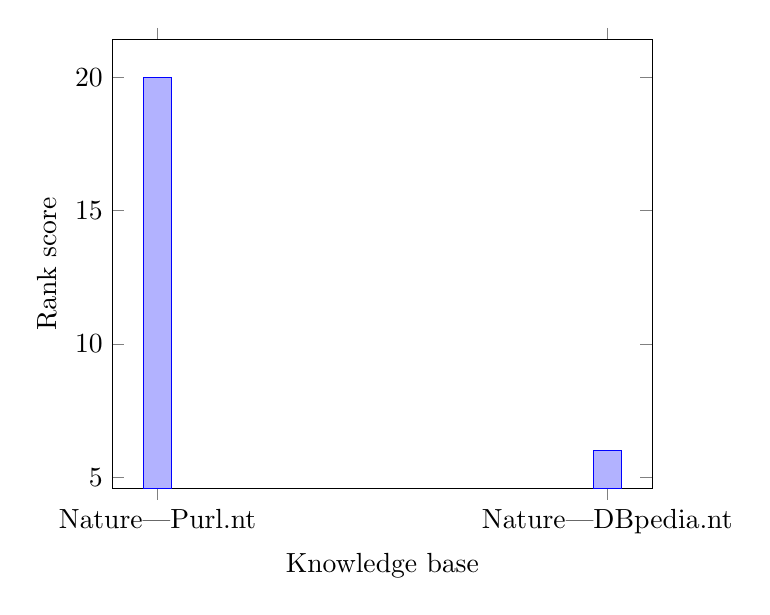
\begin{tikzpicture}
		\begin{axis}[
		scale=1.0,
		%ymode = log,
		ybar,
		xlabel={Knowledge base},
		ylabel={Rank score},
		symbolic x coords={Nature---Purl.nt,Nature---DBpedia.nt},
		xtick=data,
		]
		%\addplot coordinates { (K1,20)(K2,6)};
		\addplot coordinates { (Nature---Purl.nt,20)(Nature---DBpedia.nt,6)};
		\end{axis}
		\end{tikzpicture}
		\label{fig:a1}
	}
	%\caption{Error rank (legends: see table \ref{tab:legends}).}
	\caption{Error rank, where Nature---Purl.nt represent the file with links between Nature and Purl.org and Nature---DBpedia.nt represent the links between Nature and DBpedia}
	\label{fig:ErrorCounts}
\end{figure}



% \begin{table}[H]
% 	\small
% 	\centering
% 	\caption{Legend for the figure \ref{fig:ErrorCounts}}
% 	\label{tab:legends}
% 	\begin{tabular}{llll}
% 		K1  & npg-core-any-linkset.nq.nt---purl.org.nt    \\
% 		K2  & npg-journals-dbpedia-linkset.nq.nt---dbpedia.org.nt
% 	\end{tabular}
% \end{table}
%
According to our rank, the knowledge-base with more errors comes from $npg-core-any-linkset.nq.nt---purl.org.nt$ with $25$ links per mapping, in which we found $20$ erroneous resource candidates. The knowledge base with fewer errors was $npg-journals-dbpedia-linkset.nq.nt---dbpedia.org.nt$ with $94$ links per mapping, in which we found $6$ erroneous resource candidates and a sum of score of $3$.

\subsubsection{Analyzing and Fixing the problems}
We use an example from CEDAL output file\footnote{\url{https://github.com/firmao/CEDAL/blob/master/CEDALEducation/output.csv}} to show how to fix a Linkset. Among the errors detected we choose the linkset file $npg-core-any-linkset.nq.nt$, in which has a case where $2$ error candidates that are transitive and are in the same dataset. In this case, we have an error type 2, where the following resource \url{http://dbpedia.org/resource/Cell_Death_and_Differentiation} is duplicated within the DBpedia dataset. 

%As CEDAL only detect the erroneous link candidates, thanks to the help of an specialist on the education area, that is a co-author of this work, was possible to fix all the problems with the linksets, in which a example of error type 2 is shown at figure \ref{fig:outEx}.

% \begin{figure}[H] 
% 	\centering
% 	\includegraphics[width=2.0\linewidth]{img/CEDALEducationResults.pdf}
% 	\caption{Example of erroneous candidate detected in Nature dataset.}
% 	\label{fig:outEx}
% \end{figure} 
%available here\footnote{\url{PUT THE ADDRESS HERE}}. 

\subsection{Conclusion and future work}
In this paper, we use an approach dubbed CEDAL in order to assess consistency problems inside linkset repositories from the educational area. CEDAL allows detecting potential causes of errors, for example, the linkset, the underlying dataset(s) and the graph path where the problem subsists.
To evaluate the approach, we selected $1049$ transitive links using datasets from Nature.com and Educational Programs. Our results showed that $20$ links we considered are erroneous.
We show a scenario where is possible to see how fragile is the educational linked data and a way to improve it detecting consistency problems.
As future work we will apply this approach to more educational linked data, extend CEDAL to work with more link types and provide a usability study.